\documentclass[oneside]{ausarbeitung}
\bibliography{latexlit}

\usepackage{adjustbox} % Für die Anpassung der Tabelle an die Seitenbreite
\usepackage{geometry} % Für die Seitenränder
\usepackage{listings}

% ----------------------------------------------------------------------

\begin{document}

%--- Sprachauswahl
% Erlaubte Werte:
%   \selectlanguage{english}
%   \selectlanguage{ngerman}
\selectlanguage{ngerman}

%--- Art der Arbeit
% Erlaubte Werte:
%   \Praxissemesterbericht
%   \Projektbericht
%   \Bachelorarbeit
%   \Seminararbeit
%   \Masterarbeit

\Projektbericht

%--- Studiengang:
% Erlaubte Werte:
%   \Informatik
%   \Elektronik
%   \DataScience
\MLD

\title{Analyse von OBD-2-Fahrzeugdaten durch maschinelles Lernen für ein optimiertes Fahrerlebnis}

\author{Nils Ostertag}
\matrikelnr{75217}

%--- Ist der Erstbetreuer (\examinerA) an der Hochschule ein Professor?
% Erlaubte Werte:
%   \examinerIsAProfessortrue   % Ja
\examinerIsAProfessorfalse  % Nein
%   \examinerIsAProfessortrue   % Ja

%--- Betreuer
\examinerA{Dr.~Marc~Hermann}
%\examinerB{Prof.~Dr.~Ulrich~Klauck}

%--- Einreichungsdatum
\date{15. August 2024}

%--- Angaben zur Firma
% Auskommentieren, wenn die Arbeit nicht bei einer ext. Firma gemacht wurde.
%\companyname{Beispielfirma}
%\industrialsector{Beispielbranche}
%\department{Beispielabteilung}
%\companystreet{Beispielstr. 1}
%\companycity{12345 Musterstadt}

%--- Angaben zum Betreuer bei dieser Firma
%\advisorname{Name des Betreuers}
%\advisorphone{(01234) 567-890}
%\advisoremail{name@company.xxx}

%--- Titelseite Anzeigen
\maketitle
\cleardoublepage

%---
\pagenumbering{roman}
\setcounter{page}{1}

%--- Firmendaten Anzeigen
% Auskommentieren, wenn die Arbeit nicht bei einer ext. Firma gemacht wurde.
%\makeworkplace
%\cleardoublepage

%--- Eidesstattliche Erklärung anzeigen
\makeaffirmation
\cleardoublepage

%---
\begin{abstract}
  
\end{abstract}
%-----------------------------------------------------------------------
\cleardoublepage
\tableofcontents

%---
\listoffigures

%---
\listoftables

%---
\lstlistoflistings

%---
\listofabbreviations
\begin{acronym}[Bsp.]  % Längstes Kürzel in der nachfolgenden
                       % Liste um die Breite der Spalte für die
                       % Abkürzungen zu bestimmen.

%% Eintrag: \acro{Referenzname}[Kürzel]{Langform}
%% Im Text wird die Abkürzung dann mit \ac{Referenzname} benutzt.
\acro{rup}[RUP]{Rational Unified Process}
%\acro{bsp}[Bsp.]{Beispiel}
\end{acronym}
%---


\cleardoublepage
\pagenumbering{arabic}
\setcounter{page}{1}

% ----------------------------------------------------------------------
\chapter{Einleitung}
\label{cha:einleitung}

Im Zuge der Digitalisierung und Vernetzung im Automobilsektor gewinnt die Analyse von Fahrzeugdaten zunehmend an Bedeutung. Eine der wichtigsten Technologien in diesem Bereich ist die On-Board-Diagnose (OBD-2), die eine Fülle an Daten über den Zustand und die Leistung von Fahrzeugen liefert. Diese Daten bieten eine wertvolle Grundlage für die Entwicklung intelligenter Systeme, die das Fahrerlebnis optimieren und die Fahrzeugwartung verbessern können. Dabei spielt das maschinelle Lernen eine zentrale Rolle, da es die Fähigkeit besitzt, Muster in den Daten zu erkennen und daraus Schlüsse zu ziehen, die für den Fahrer von großem Nutzen sein können.

\section{Problemstellung und -abgrenzung}
\label{sec:problemstellung}

Trotz der Vorteile, die OBD-2-Daten und maschinelles Lernen bieten, bleibt die effiziente Nutzung dieser Technologien eine Herausforderung. Die schiere Menge und Komplexität der erhobenen Daten erschweren es, aussagekräftige und nützliche Informationen für den Endnutzer abzuleiten. Zudem variieren die Anforderungen an die Fahrstilanalyse je nach Fahrzeugtyp und individuellen Nutzungsgewohnheiten, was eine maßgeschneiderte Analyse notwendig macht. Bisherige Ansätze fokussieren sich oft nur auf spezifische Aspekte wie die Fehlerdiagnose oder den Kraftstoffverbrauch, lassen jedoch eine ganzheitliche Bewertung des Fahrstils und der Fahrzeugnutzung vermissen.
Ein weiteres Problem ist die Integration der gewonnenen Erkenntnisse in ein nutzerfreundliches System, das dem Fahrer verständliche und umsetzbare Empfehlungen gibt. Ohne eine klare und präzise Aufbereitung der Daten besteht die Gefahr, dass die Ergebnisse der Analyse für den Nutzer schwer verständlich oder gar nutzlos werden. Die Abgrenzung dieser Arbeit liegt darin, den Fokus auf die Entwicklung eines umfassenden Algorithmus zu legen, der verschiedene Aspekte des Fahrverhaltens in Echtzeit analysiert und dem Nutzer in einfacher Form präsentiert.

\section{Ziel der Arbeit}
\label{sec:ziel}

Das Ziel dieser Arbeit ist es, OBD-2-Datensätze zur Bewertung und Optimierung des Fahrstils eines Nutzers zu verwenden. Hierbei sollen Algorithmen des maschinellen Lernens zum Einsatz kommen, um kritische Aspekte wie Kraftstoffverbrauch, Fahrzeugleistung und Verschleißprävention zu bewerten. Ein weiterer Schwerpunkt liegt auf der frühzeitigen Erkennung potenzieller Probleme, um präventive Maßnahmen empfehlen zu können. Am Ende der Arbeit soll ein Algorithmus entwickelt werden, der dem Nutzer nicht nur Rückmeldungen über seinen aktuellen Fahrstil gibt, sondern auch Optimierungsmöglichkeiten aufzeigt, die zu einem effizienteren und sichereren Fahrerlebnis führen. Dieses System soll langfristig dazu beitragen, die Lebensdauer des Fahrzeugs zu verlängern und die Wartungskosten zu senken, indem es dem Nutzer datenbasierte Einblicke in den Zustand seines Fahrzeugs und seinen Fahrstil liefert.

\section{Vorgehen}
\label{sec:vorgehen}

% ---

\chapter{Aktueller Forschungsstand}
\label{cha:forschungsstand}

\section{Fahrverhaltensanalyse}
\label{sec:research_fahrverhalten}

Die Analyse von OBD-2-Fahrzeugdaten mittels maschinellen Lernens hat sich in den letzten Jahren als bedeutender Forschungsschwerpunkt etabliert. OBD-2 (On-Board-Diagnose) bietet eine standardisierte Schnittstelle zur Überwachung und Analyse zahlreicher Fahrzeugparameter in Echtzeit. Diese Technologie hat das Potenzial, durch die Integration mit maschinellen Lernalgorithmen nicht nur Fahrzeugdiagnosen zu verbessern, sondern auch das Fahrerlebnis und die Effizienz des Fahrstils maßgeblich zu optimieren.

Eine zentrale Anwendung des maschinellen Lernens in diesem Bereich ist die Klassifikation von Fahrverhalten. Hierbei werden verschiedene Algorithmen wie Support Vector Machines (SVM), AdaBoost und Random Forest eingesetzt, um Fahrstile anhand von Parametern wie Kraftstoffverbrauch, Lenkradstabilität, Geschwindigkeitsstabilität und Bremsverhalten zu klassifizieren. Diese Modelle erzielen dabei eine hohe Genauigkeit, was ihre Eignung für die Bewertung und Verbesserung des Fahrverhaltens unterstreicht [10
.pdf].
Die Analyse und Klassifikation des Fahrverhaltens erfolgt typischerweise durch die Erfassung von Daten über das OBD-2-Protokoll. Diese Daten umfassen eine Vielzahl von Sensorwerten, wie Motordrehzahl, Gaspedalstellung und Fahrzeuggeschwindigkeit. Maschinelle Lernverfahren nutzen diese Daten, um individuelle Fahrmuster zu identifizieren und potenzielle Verbesserungsmöglichkeiten aufzuzeigen. Ein Beispiel für die Anwendung solcher Verfahren ist die Entwicklung von Modellen zur Abschätzung des Fahrmodus basierend auf den über das OBD-2-Protokoll erfassten PID-Signalen (Parameter IDs). Diese Modelle ermöglichen es, das Fahrverhalten in Echtzeit zu analysieren und Optimierungen vorzuschlagen, die sowohl die Sicherheit als auch die Effizienz des Fahrens verbessern [9
.pdf].
Zusätzlich zur Verhaltensanalyse hat sich das maschinelle Lernen auch als Werkzeug zur Diagnose und Wartung von Fahrzeugen etabliert. Durch die Analyse der OBD-2-Daten können potenzielle Probleme frühzeitig erkannt und präventive Wartungsmaßnahmen vorgeschlagen werden, was langfristig zur Reduzierung von Betriebskosten und zur Verbesserung der Fahrzeugleistung beiträgt. Diese Ansätze bieten nicht nur einen direkten Nutzen für den Endnutzer, sondern können auch in Bereichen wie der Flottenverwaltung oder der Versicherungswirtschaft eingesetzt werden, um das Risikomanagement zu optimieren und maßgeschneiderte Versicherungsprämien zu berechnen [10
.pdf].

Insgesamt zeigt der aktuelle Forschungsstand, dass die Kombination von OBD-2-Technologie und maschinellem Lernen weitreichende Möglichkeiten zur Verbesserung des Fahrerlebnisses und der Fahrzeugwartung bietet. Die kontinuierliche Weiterentwicklung dieser Technologien wird voraussichtlich zu noch präziseren und effektiveren Lösungen führen, die sowohl die Sicherheit als auch die Effizienz im Straßenverkehr erhöhen.


% ---
\chapter{Theoretische Grundlagen}
\label{cha:grundlagen}

Dieses Kapitel bildet das Fundament für das Verständnis der in dieser Arbeit behandelten Konzepte und Methoden. Es stellt die notwendigen theoretischen Konzepte und technischen Grundlagen vor, die für die Analyse von OBD-2-Fahrzeugdaten und den Einsatz von maschinellen Lernverfahren relevant sind. Zunächst werden die Funktionsweise und Struktur der OBD-2-Technologie erläutert, gefolgt von einer Einführung in die grundlegenden Prinzipien der Fahrstilcharacterisierung. Anschließend werden weitere Grundlagen vermittelt, die für das Verständnis von Subkomponenten des Gesamtsystems notwendig sind. Diese theoretischen Grundlagen sind essenziell, um die späteren Analysen und Algorithmen in den Kontext der aktuellen Forschung einzuordnen und deren Anwendung auf reale Fahrzeugdaten zu ermöglichen.

\section{OBD-II}
\label{sec:foundations_obd2}

\subsection*{Einführung in die On-Board-Diagnose II}
\label{subsec:foundations_obd2_intro}
Die On-Board-Diagnose II (OBD-II) ist ein standardisiertes System, das zur Überwachung der Funktionalität von Fahrzeugkomponenten entwickelt wurde. Sie ermöglicht es, Informationen über den Zustand eines Fahrzeugs zu erhalten und potenzielle Probleme frühzeitig zu identifizieren. Bereits ab August 1965 begann Volkswagen, die produzierten Fahrzeuge mit einer Zentralsteckdose auszustatten, die über einen Diagnosestecker mit einem lochkartengesteuerten Rechnersystem verbunden werden konnte [Wikipedia]. Der Zweck dieser Einrichtung bestand in der automatisierten Diagnose in Werkstätten, wobei die Abgasdiagnose damals noch nicht Bestandteil des Untersuchungsprogramms war.

Die Einführung von OBD-Systemen speziell für die Abgasdiagnose erfolgte im Jahr 1988 durch das kalifornische California Air Resources Board (CARB, dt. etwa „Luftreinhalte-Behörde“) in den USA. Diese Maßnahme markierte den Beginn der Entwicklung moderner OBD-Systeme, die sich mit der Überwachung und Steuerung der Fahrzeugemissionen befassen. OBD-II wurde schließlich 1996 in den USA verpflichtend eingeführt und ist seitdem in den meisten modernen Fahrzeugen weltweit integriert.

Der OBD-II-Standard umfasst sowohl die Hardware- als auch die Softwarekomponenten, die für die Fahrzeugdiagnose notwendig sind. Ein zentraler Bestandteil des Systems ist der standardisierte Diagnosestecker, der sogenannte Diagnostic Link Connector (DLC), der in der Regel unter dem Armaturenbrett des Fahrzeugs zu finden ist. Dieser 16-polige Stecker ermöglicht den Zugriff auf verschiedene elektronische Steuergeräte (ECUs) im Fahrzeug, die wiederum eine Vielzahl von Sensordaten erfassen und speichern. Über diesen Stecker kann ein OBD-II-Scanner mit dem Fahrzeug verbunden werden, um Diagnosedaten auszulesen, Fehlercodes zu identifizieren und gegebenenfalls zu löschen.

\begin{figure}[h!]
  \centering
  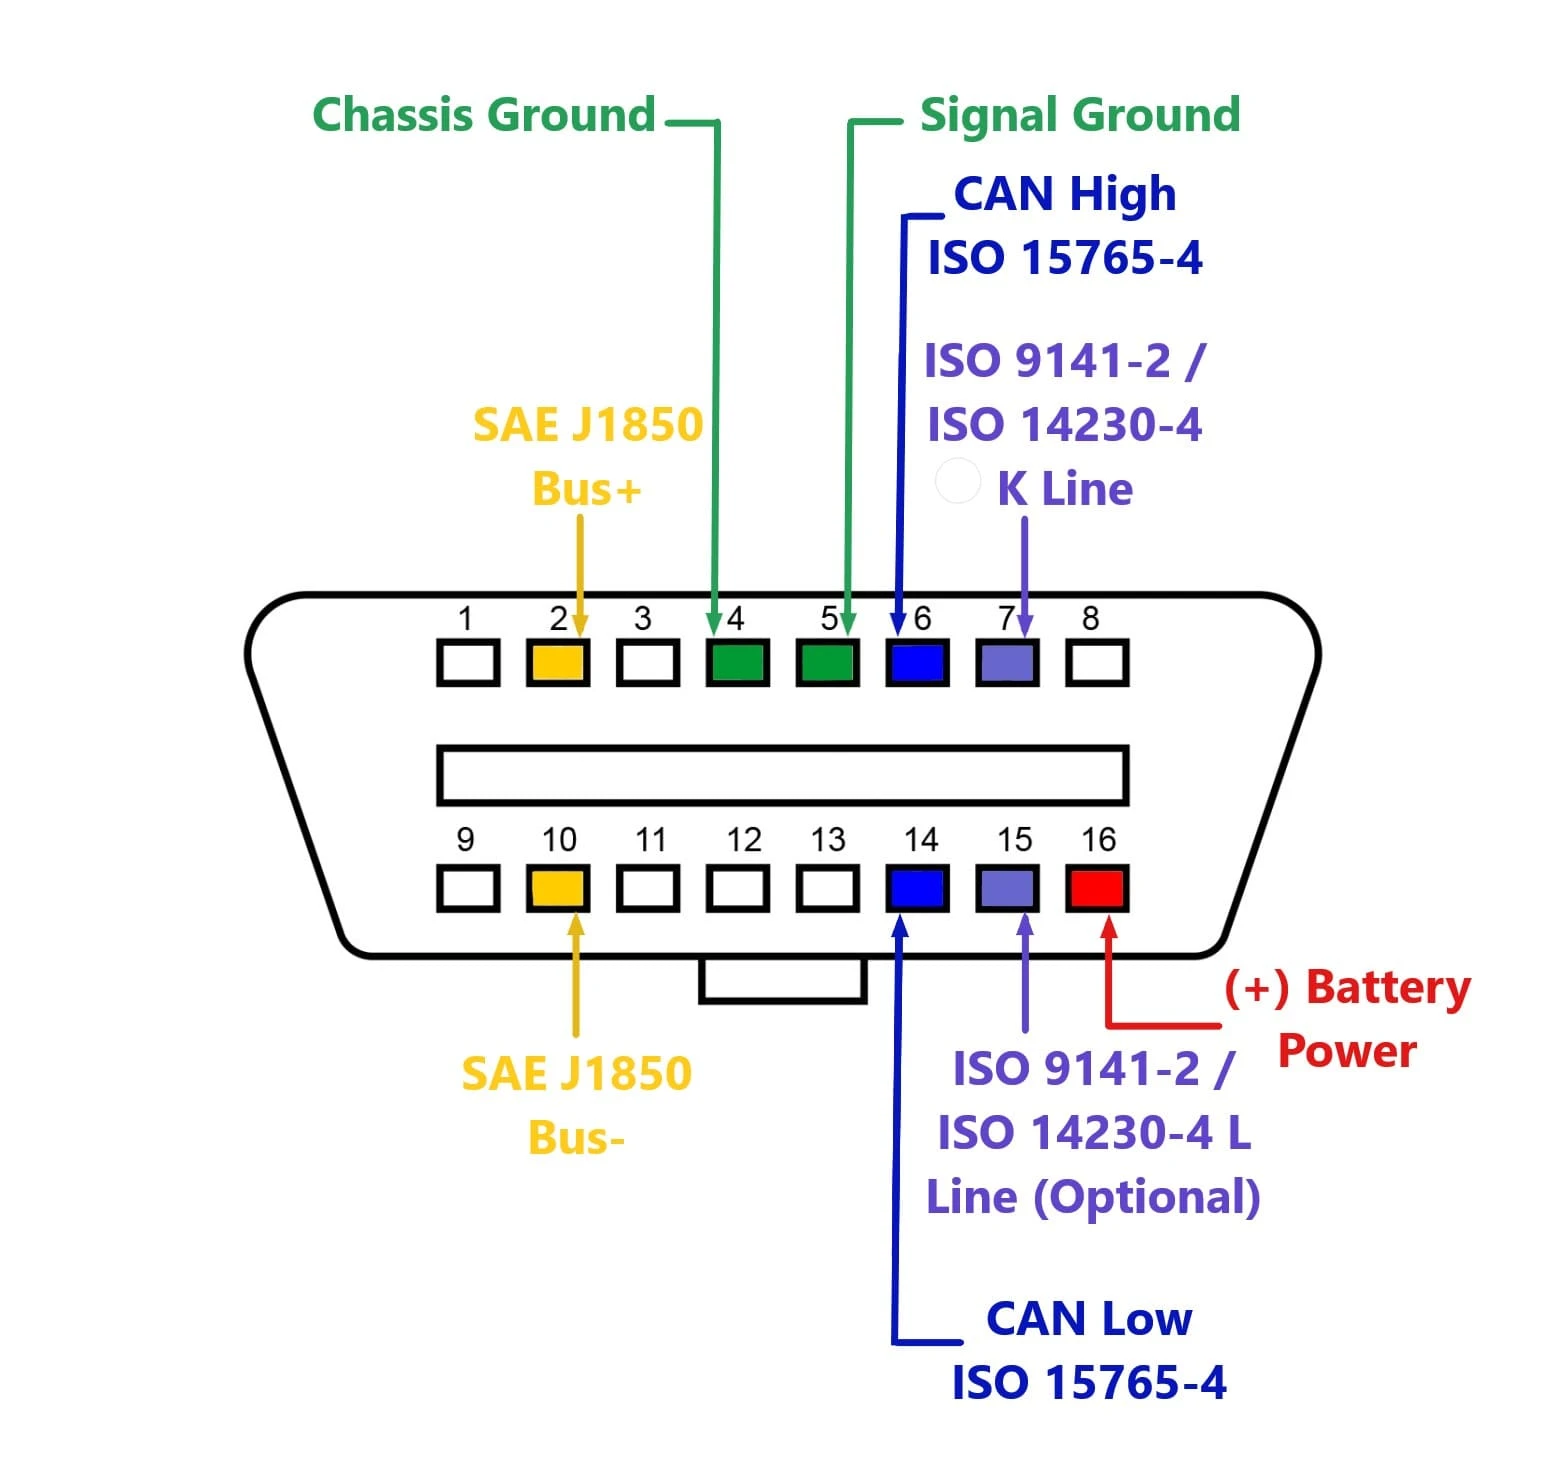
\includegraphics[width=0.75\textwidth]{images/pinout_explanation.png}
  \caption{Übersicht zur OBD-II Pinbelegung}
  \label{fig:obd2_pinout}
\end{figure}
%https://www.flexihub.com/images/upload/flexihub/articles/diagnostics/pinout_explanation.jpg

Ein wesentlicher Bestandteil der OBD-II-Technologie ist das Protokollsystem, das die Kommunikation zwischen dem Fahrzeug und dem Diagnosegerät regelt. Es gibt mehrere Kommunikationsprotokolle, die je nach Fahrzeughersteller variieren können. Zu den am häufigsten verwendeten Protokollen gehören das Controller Area Network (CAN), ISO 9141-2, KWP2000 und SAE J1850. Das CAN-Bus-Protokoll, das von Bosch entwickelt wurde, ist das am weitesten verbreitete und ermöglicht eine schnelle und zuverlässige Datenübertragung zwischen den verschiedenen Steuergeräten im Fahrzeug.

\begin{table}[h!]
  \centering
  \begin{adjustbox}{width=\textwidth}
  \begin{tabular}{|l|l|l|l|}
  \textbf{Protokoll} & \textbf{PIN-Belegung DLC} & \textbf{Geschwindigkeit} & \textbf{Verwendung} \\ 
  SAE J1850 PWM & PIN 2, PIN 10 & 41.6 kbit/s & Vorwiegend in Ford-Fahrzeugen \\ 
  SAE J1850 VPW & PIN 2 & 10.4 kbit/s & Vorwiegend in GM-Fahrzeugen \\ 
  ISO 9141-2 & PIN 7, PIN 15 & 10.4 kbit/s & Europäische und asiatische Fahrzeuge \\ 
  ISO 14230-4 (KWP2000) & PIN 7, PIN 15 & 10.4 kbit/s & Europäische und asiatische Fahrzeuge \\ 
  ISO 15765-4 (CAN-Bus) & PIN 6, PIN 14 & 250 kbit/s oder 500 kbit/s & Fahrzeuge ab BJ 2008 \\ 
  \end{tabular}
  \end{adjustbox}
  \caption{Übersicht zu gängigen OBD-II-Protokollen}
  \label{tab:obd_protocols}
\end{table}

Der OBD-II-Standard umfasst verschiedene Diagnosemodi, die es ermöglichen, unterschiedliche Arten von Fahrzeugdaten auszulesen. Mode 1 beispielsweise erlaubt den Echtzeitzugriff auf Sensordaten wie Geschwindigkeit, Motordrehzahl, Temperatur und Druckverhältnisse. Mode 3 dient zum Auslesen von gespeicherten Fehlercodes (DTCs), die auf spezifische Probleme im Fahrzeug hinweisen. Mit Mode 4 können diese Fehlercodes und die damit verbundenen Daten gelöscht werden.

Ein wichtiges Merkmal der OBD-II-Technologie ist ihre Fähigkeit, eine Vielzahl von Fahrzeugen unterschiedlicher Marken und Modelle zu unterstützen. Dies wird durch die Standardisierung der PIN-Belegung des DLC-Steckers und die Verwendung universeller Protokolle erreicht. Die Integration von OBD-II in Fahrzeuge ermöglicht es nicht nur Werkstätten, sondern auch Fahrzeugbesitzern, Diagnosen durchzuführen und grundlegende Informationen über den Zustand ihres Fahrzeugs zu erhalten. Besonders populär sind kostengünstige OBD-II-Scanner, die in Verbindung mit einer Smartphone-App genutzt werden können, um Diagnosedaten in Echtzeit abzurufen.

\subsection*{ELM-327}
\label{subsec:foundations:elm327}
Das ELM327-Modul ist ein weitverbreitetes Interface, das speziell für die Kommunikation mit dem On-Board-Diagnose-System der zweiten Generation (OBD2) entwickelt wurde. Es fungiert als Brücke zwischen einem Fahrzeug und einem externen Gerät wie einem Computer, Smartphone oder einem speziellen Diagnosegerät. Der Hauptzweck des ELM327 ist es, Fahrzeugdaten zu lesen und zu analysieren, um Probleme im Fahrzeug zu diagnostizieren und zu überwachen.

Der ELM327-Chipsatz basiert auf einem Mikrocontroller, der verschiedene Kommunikationsprotokolle unterstützt, die in Fahrzeugen mit OBD2-Standard verwendet werden. Dazu gehören unter anderem ISO9141, KWP2000, J1850 PWM, J1850 VPW und CAN-Bus, was ihn äußerst vielseitig für den Einsatz in unterschiedlichen Automarken und -modellen macht (ELM327DSH.pdf). Die Verbindung zu einem Fahrzeug erfolgt in der Regel über den OBD2-Port, der sich meist unter dem Armaturenbrett befindet. Sobald der ELM327 an diesen Port angeschlossen ist, kann er die Signale des Fahrzeugs interpretieren und an ein verbundenes Gerät weiterleiten.

Ein wesentlicher Vorteil des ELM327 liegt in seiner Fähigkeit, auf Echtzeitdaten des Fahrzeugs zuzugreifen. Dazu gehören Motordrehzahlen, Fahrzeuggeschwindigkeit, Kühlmitteltemperatur, Luftmassenstrom und viele weitere Parameter, die über die standardisierten PIDs (Parameter IDs) abgerufen werden können. Diese Daten können dann entweder in einer simplen Textform angezeigt oder in detaillierte Graphen umgewandelt werden, die dem Benutzer helfen, ein tieferes Verständnis der Fahrzeugleistung zu entwickeln (USING\_OBD-2\_TECHNOLOGY\_FOR\_VEHICLE\_DIAGNOSTIC\_AND\_.pdf).

Ein weiterer bedeutender Aspekt des ELM327 ist seine Fähigkeit zur Fehlerdiagnose. Der ELM327 kann Fehlercodes (DTCs) auslesen, die von der Motorsteuerung (ECU) gespeichert wurden. Diese Codes geben Hinweise auf spezifische Probleme oder Störungen im Fahrzeug. Zusätzlich zu den generischen Fehlercodes, die markenübergreifend standardisiert sind, kann der ELM327 auch herstellerspezifische Codes auslesen, was eine präzisere Diagnose ermöglicht. Ein Benutzer kann diese Fehlercodes dann interpretieren und gegebenenfalls entsprechende Maßnahmen ergreifen, wie z.B. die Durchführung von Reparaturen oder die Rücksetzung der Motorleuchte (ELM327DSH.pdf).

Der ELM327 hat sich als ein unverzichtbares Werkzeug für sowohl Hobbyisten als auch professionelle Mechaniker etabliert, da er eine kostengünstige und benutzerfreundliche Lösung für die Fahrzeugdiagnose bietet. Die Möglichkeit, ihn mit einer Vielzahl von Software-Tools und Apps zu verbinden, erweitert seine Einsatzmöglichkeiten erheblich. Ob zur Überwachung von Fahrzeugleistungen, zur Fehlersuche oder zur Datenerfassung – der ELM327 stellt eine flexible und leistungsstarke Schnittstelle dar, die den Zugang zu wichtigen Fahrzeuginformationen ermöglicht und damit einen entscheidenden Beitrag zur Fahrzeugwartung und -diagnose leistet.

Durch die kontinuierliche Weiterentwicklung und Verbesserung der Firmware bleibt der ELM327 ein zukunftssicheres Werkzeug, das sich an die ständig wachsenden Anforderungen der Fahrzeugdiagnose anpasst (USING\_OBD-2\_TECHNOLOGY\_FOR\_VEHICLE\_DIAGNOSTIC\_AND\_.pdf).

\section{Fahrverhalten und -Charakteristiken}
\label{sec:foundations_fahrverhalten}

\section{Node-RED}
\label{sec:foundations_nodered}
Node-RED ist ein Open-Source-Framework, das für die visuelle Programmierung entwickelt wurde, um das Rapid Prototyping von Anwendungen und das schnelle Entwickeln von Backend-Anwendungen zu erleichtern. Es basiert auf der JavaScript-Laufzeitumgebung Node.js und ermöglicht es Benutzern, Anwendungen durch das Verknüpfen von "Nodes" zu erstellen, die unterschiedliche Funktionen und Datenflüsse repräsentieren. Node-RED verwendet ein browserbasiertes Interface, das es Entwicklern ermöglicht, durch Drag-and-Drop-Methoden eine Vielzahl von Funktionen zu integrieren und zu orchestrieren.

Das Framework ist besonders gut geeignet für den Einsatz auf kleinen, ressourcenbegrenzten Geräten wie dem Raspberry Pi, einem beliebten Einplatinencomputer. Die Integration von Node-RED auf einem Raspberry Pi bietet eine kostengünstige und leistungsfähige Plattform für Rapid Prototyping und die Entwicklung von Backend-Systemen. Der Raspberry Pi, ausgestattet mit einer ARM-basierten CPU und ausreichendem Arbeitsspeicher für leichte bis mittlere Lasten, stellt eine ideale Umgebung für Node-RED bereit, da es die Flexibilität und Skalierbarkeit der Plattform unterstützt, während es gleichzeitig geringe Hardwareanforderungen hat.

Node-RED auf dem Raspberry Pi kann verwendet werden, um verschiedene Backend-Anwendungen zu entwickeln, wie zum Beispiel IoT-Systeme, Datenverarbeitungspipelines und Automatisierungsanwendungen. Der visuelle Programmieransatz von Node-RED ermöglicht es Entwicklern, komplexe Datenflüsse zu modellieren und zu steuern, indem sie einfache Knoten für verschiedene Aufgaben wie HTTP-Anfragen, Datenbankinteraktionen oder Echtzeitkommunikation nutzen. Diese Knoten können mit minimalem Codeaufwand konfiguriert und kombiniert werden, um maßgeschneiderte Lösungen zu erstellen.

Durch die Verwendung von Node-RED auf einem Raspberry Pi können Entwickler schnell Prototypen erstellen und testen, da das Framework eine reiche Sammlung von vorgefertigten Knoten bietet, die für unterschiedliche Protokolle und Dienste wie MQTT, WebSockets, und Datenbanken optimiert sind. Diese Knoten erleichtern die Integration und Interaktion mit verschiedenen Hardwarekomponenten und Online-Diensten. Darüber hinaus unterstützt Node-RED die Entwicklung benutzerdefinierter Knoten, was es ermöglicht, spezifische Funktionen und Anpassungen schnell zu integrieren, um die Anforderungen des Prototypen zu erfüllen.

\section{InfluxDB}
\label{sec:foundations_influxdb}

InfluxDB ist eine hochleistungsfähige, Open-Source-Datenbank, die speziell für die Speicherung und Abfrage von Zeitreihendaten entwickelt wurde. Zeitreihendaten sind Daten, die in einem zeitlichen Kontext erfasst werden, wie zum Beispiel Temperaturmessungen über den Tag oder Servermetriken im Laufe der Zeit. Was InfluxDB besonders auszeichnet, ist seine Optimierung für die effiziente Handhabung großer Mengen solcher Daten in Echtzeit.

Ein zentrales Merkmal von InfluxDB ist seine Architektur, die speziell für Zeitreihendaten entwickelt wurde. Im Gegensatz zu traditionellen relationalen Datenbanken, die auf Tabellen und Zeilen basieren, verwendet InfluxDB ein Schema-freies Modell, das für die flexible Speicherung und Abfrage von Zeitstempeln und zugehörigen Werten optimiert ist. Diese Struktur erlaubt es, Daten schnell und effizient zu speichern, insbesondere wenn es um hohe Schreib- und Lesevolumen geht.

InfluxDB implementiert ein komprimiertes Speichermodell, das sowohl die Datenmenge reduziert als auch die Geschwindigkeit der Datenabfragen erhöht. Es nutzt eine Methode namens "Time-Structured Merge Tree" (TSM Tree), um Daten effizient zu organisieren und zu speichern. Die TSM-Bäume ermöglichen eine schnelle Datenkompression und -dekompression sowie eine zügige Aggregation von Zeitreihendaten.

Ein weiteres hervorhebenswertes Feature ist die Unterstützung der Abfragesprache InfluxQL, die SQL-ähnlich ist und es Nutzern ermöglicht, komplexe Zeitreihenanalysen durchzuführen. Ab Version 2.0 hat InfluxDB auch Flux eingeführt, eine leistungsfähige Abfragesprache und Skriptsprache, die noch mehr Flexibilität bei der Datenmanipulation und -analyse bietet.

Darüber hinaus bietet InfluxDB eingebaute Funktionen zur Datenaggregation und -analyse, wie zum Beispiel kontinuierliche Abfragen, die es ermöglichen, aggregierte Daten in Echtzeit zu berechnen und zu speichern. Diese kontinuierlichen Abfragen können verwendet werden, um regelmäßig aktualisierte Metriken oder Statistiken zu erstellen, ohne dass zusätzliche Verarbeitungsschritte erforderlich sind.

Die Integration von InfluxDB in verschiedene Überwachungs- und Analysetools sowie seine Fähigkeit, große Datenmengen in Echtzeit zu verarbeiten, machen es zu einer bevorzugten Wahl für Anwendungsfälle wie Infrastrukturüberwachung, IoT-Datenanalyse und Anwendungsleistungsmanagement.

\section{WireGuard VPN}
\label{sec:foundations_wireguard}
WireGuard ist ein modernes Virtual Private Network (VPN)-Protokoll, das aufgrund seiner Einfachheit und Sicherheit zunehmend an Bedeutung gewinnt. Entwickelt von Jason A. Donenfeld, zeichnet sich WireGuard durch seine hohe Effizienz, einfache Implementierung und starke Kryptografie aus. Im Vergleich zu älteren VPN-Protokollen wie IPsec oder OpenVPN bietet WireGuard eine wesentlich schlankere Codebasis, was nicht nur die Sicherheitsüberprüfung erleichtert, sondern auch die Performance verbessert.

WireGuard verwendet moderne Kryptografiebibliotheken und -techniken, um sichere Kommunikationskanäle zwischen zwei Endpunkten zu etablieren. Es basiert auf dem Konzept der "Public Key Authentication", bei dem jeder Teilnehmer einen privaten und einen öffentlichen Schlüssel besitzt. Die Authentifizierung und Verschlüsselung erfolgen durch diese Schlüsselpaare, wobei der öffentliche Schlüssel des Gegenübers zum Aufbau einer sicheren Verbindung verwendet wird. WireGuard nutzt dafür die Verschlüsselungsalgorithmen Curve25519 für die elliptische Kurven-Schlüsselaustausch, ChaCha20 für die Verschlüsselung der Daten, Poly1305 für die Datenintegrität und BLAKE2 für die Hash-Funktion. Diese moderne kryptografische Grundlage stellt sicher, dass die Verbindungen sowohl sicher als auch effizient sind.

Die Implementierung von WireGuard auf Embedded Systems wie dem Raspberry Pi ist besonders interessant, da dieser Computer in der Lage ist, als kostengünstiger und energieeffizienter VPN-Server zu fungieren. Der Raspberry Pi ist ein weit verbreitetes Embedded-System, das aufgrund seiner geringen Größe und Leistungsmöglichkeiten gut für solche Aufgaben geeignet ist.

Um WireGuard auf einem Raspberry Pi einzurichten, folgen im Allgemeinen mehrere Schritte. Zunächst muss das Raspberry Pi Betriebssystem, typischerweise eine Distribution wie Raspberry Pi OS, auf dem Gerät installiert sein. Nachdem das System eingerichtet und auf dem neuesten Stand ist, kann WireGuard installiert werden. Dies geschieht in der Regel durch den Paketmanager des Betriebssystems, z.B. durch den Befehl sudo apt-get install wireguard.

Nach der Installation sind die nächsten Schritte die Konfiguration von WireGuard. Hierbei wird eine Konfigurationsdatei erstellt, die die notwendigen Parameter wie private und öffentliche Schlüssel, sowie die Netzwerkschnittstellen beschreibt. Auf dem Raspberry Pi wird üblicherweise ein wg0 Interface erstellt, welches die VPN-Verbindung darstellt. Die Konfiguration umfasst auch die Definition der IP-Adressen, die den VPN-Teilnehmern zugewiesen werden, sowie die Routen, die durch das VPN geleitet werden sollen.

Ein wichtiger Aspekt bei der Verbindung zum Heimnetzwerk über ein VPN ist das Routing der Daten. Um von einem entfernten Standort auf das Heimnetzwerk zugreifen zu können, muss das Routing so konfiguriert sein, dass der Datenverkehr vom VPN-Client über den Raspberry Pi und dann ins lokale Netzwerk weitergeleitet wird. Dies erfordert oft zusätzliche Konfigurationen wie das Aktivieren des IP-Forwardings und das Einrichten entsprechender Firewall-Regeln auf dem Raspberry Pi.

\section{App-Development mit Flutter}
\label{sec:foundations_flutter}

Flutter ist ein Open-Source-Framework für die App-Entwicklung, das von Google entwickelt wurde und sich durch eine Vielzahl einzigartiger Eigenschaften auszeichnet. Es ermöglicht Entwicklern, nativ kompilierte Anwendungen für mobile, Web- und Desktop-Plattformen aus einer einzigen Codebasis zu erstellen. Die Kerntechnologie von Flutter basiert auf der Programmiersprache Dart, die ebenfalls von Google entwickelt wurde. Dart bietet eine moderne, objektorientierte Syntax und ist darauf ausgelegt, schnelle Entwicklungszyklen zu unterstützen.

Ein zentrales Merkmal von Flutter ist die Verwendung einer eigenen Rendering-Engine, die als Skia bezeichnet wird. Diese Engine ermöglicht es Flutter, grafische Inhalte direkt auf den Bildschirm zu zeichnen, ohne auf die nativen UI-Komponenten der jeweiligen Plattform angewiesen zu sein. Dies bedeutet, dass Entwickler die volle Kontrolle über das Layout und das Aussehen der Benutzeroberfläche haben, was zu einer hohen Konsistenz und Flexibilität in der Gestaltung führt. Die direkte Zeichnung auf der Skia-Engine reduziert die Abhängigkeit von plattformspezifischen UI-Elementen und ermöglicht eine präzise Anpassung der Benutzeroberfläche an die Bedürfnisse der Anwendung.

Ein weiterer bedeutender Vorteil von Flutter ist das „Hot Reload“-Feature. Dieses Werkzeug erlaubt Entwicklern, Änderungen am Code in Echtzeit zu sehen, ohne die gesamte Anwendung neu starten zu müssen. Diese Fähigkeit beschleunigt den Entwicklungsprozess erheblich, da sie es Entwicklern ermöglicht, sofortige Rückmeldungen zu erhalten und Anpassungen vorzunehmen, ohne den Zustand der App zu verlieren. Dies fördert eine iterative Entwicklung und erleichtert die experimentelle Gestaltung und Fehlerbehebung.

Flutter bietet zudem eine umfangreiche Sammlung von Widgets, die die Entwicklung von ansprechenden Benutzeroberflächen vereinfachen. Diese Widgets sind in das Framework integriert und ermöglichen es Entwicklern, komplexe Benutzeroberflächen mit minimalem Aufwand zu erstellen. Die Widgets sind in einer Hierarchie organisiert und ermöglichen eine tiefgreifende Anpassung sowie die Erstellung von benutzerdefinierten Widgets, die den spezifischen Anforderungen der Anwendung entsprechen.

Ein weiteres bemerkenswertes Merkmal von Flutter ist die hohe Performance, die durch die direkte Kompilierung des Dart-Codes in native Maschinensprache erreicht wird. Dies führt zu schnelleren Startzeiten und einer flüssigen Benutzererfahrung, da der Code nicht durch eine zusätzliche Schicht wie eine virtuelle Maschine oder ein Webview interpretiert werden muss. Die Performance-Optimierung wird weiter durch die effiziente Nutzung von GPU-Beschleunigung und die Unterstützung für Hardware-gestützte Animationen verstärkt.

\section{Multi-Output Regression}
\label{sec:foundations_multioutputregression}

\subsection*{Random Forest}

%---
\chapter{Umsetzung und Implementierung}
\label{cha:implement}

\section{Anforderungsanalyse}
\label{sec:implement_requirements}

Die Anforderungsanalyse bildet das Herzstück eines erfolgreichen Projekts, da sie die Grundlage für die Entwicklung und 
Implementierung bildet. In dieser Phase wird der Rahmen für alle nachfolgenden Aktivitäten festgelegt, indem die Bedürfnisse,
Erwartungen und spezifischen Anforderungen des Projekts klar definiert werden. Diese Analyse ist von entscheidender Bedeutung, 
um sicherzustellen, dass das Endprodukt oder Ergebnis den definierten Zielen entspricht und den gewünschten Nutzen bietet.

\begin{itemize}
  \item \textbf{Data Aquisition von Fahrdaten}\\ Das erste fundamentale Ziel zur Umsetzung der Projektidee ist die Erhebung von 
  Fahrdaten in Echtzeit. Hierfür muss geklärt werden, welche spezifischen Daten erfasst werden sollen und auf welchem Weg dies 
  erfolgen soll. Neben der Wahl der Datenquellen, wie OBD-II-Schnittstellen, GPS-Modulen und weiteren Sensoren, muss auch die 
  Datenübertragungstechnologie festgelegt werden, um eine zuverlässige und effiziente Kommunikation sicherzustellen. Dies könnte 
  beispielsweise über mobile Netzwerke, WLAN oder spezielle IoT-Protokolle erfolgen. Weiterhin ist zu definieren, mit welcher 
  Frequenz die Daten erhoben und an das Backend zur Verarbeitung weitergeleitet werden, um sowohl die Datenqualität als auch die
  Systemressourcen optimal zu nutzen.
  
  Ein weiterer kritischer Aspekt ist die Integration zusätzlicher Datenquellen, die über OBD-II-Daten hinausgehen, um umfassendere
  Analysen zu ermöglichen. Dazu zählen unter anderem GPS-Daten zur genauen Standortbestimmung, UUIDs zur Identifikation einzelner 
  Fahrzeuge oder Fahrer sowie möglicherweise Umweltdaten (z.B. Wetterbedingungen). Diese zusätzlichen Daten können helfen, 
  Kontextinformationen zu den Fahrdaten zu liefern, die für präzisere Analysen und Vorhersagen unerlässlich sind.
  
  Zudem sollte auch die Datensicherheit und der Datenschutz von Anfang an berücksichtigt werden. Dies betrifft sowohl die sichere 
  Übertragung der Daten als auch deren Speicherung und Verarbeitung. Es ist essenziell, dass alle erhobenen Daten entsprechend den 
  geltenden Datenschutzbestimmungen behandelt werden und Maßnahmen zur Sicherung der Datenintegrität und -vertraulichkeit implementiert 
  werden. Schließlich sollte ein robustes Monitoring- und Wartungssystem eingerichtet werden, um die Datenakquise kontinuierlich zu überwachen und gegebenenfalls zeitnah Anpassungen vorzunehmen.
  
  \item \textbf{Datenaustausch zwischen Client und Backend}\\ Der Datenaustausch zwischen dem Client, in diesem Fall einer Mobile-App, 
  und dem Backend ist essenziell für die Funktionalität und Effizienz des gesamten Systems. Neben der reinen Datenerhebung spielt die 
  sichere und performante Übermittlung von Daten eine zentrale Rolle. Dabei ist es wichtig, Technologien zu wählen, die nicht nur eine 
  sichere Verbindung, sondern auch einen schnellen und zuverlässigen Austausch von Anfragen und Datensätzen gewährleisten.
  
  Eine wesentliche Voraussetzung für den erfolgreichen Datenaustausch ist die Definition klarer und zielorientierter Rahmenbedingungen. 
  Dazu gehören die Spezifikation der verschiedenen Anfragetypen, die Gestaltung effizienter und skalierbarer Datenstrukturen sowie die 
  Berücksichtigung der erforderlichen Flexibilität des Backends im Entwicklungsverlauf. Das Backend muss in der Lage sein, auf sich 
  ändernde Anforderungen schnell zu reagieren und gegebenenfalls neue Datenstrukturen oder Schnittstellen zu implementieren, ohne dabei 
  die Stabilität oder Sicherheit des Systems zu gefährden.
  
  Darüber hinaus spielt die Wahl der richtigen Protokolle und Authentifizierungsmechanismen eine entscheidende Rolle. Protokolle wie HTTPS 
  oder WebSocket bieten eine gute Basis für die sichere Übertragung von Daten, während Authentifizierungsverfahren wie OAuth oder JWT 
  (JSON Web Tokens) sicherstellen, dass nur autorisierte Clients Zugriff auf sensible Daten erhalten. Auch die Handhabung von Fehlern und 
  Ausnahmen im Datenaustausch sollte frühzeitig definiert werden, um eine hohe Robustheit und Benutzerfreundlichkeit der Mobile-App zu 
  gewährleisten.
  
  Schließlich ist es von Vorteil, Mechanismen zur Überwachung und Protokollierung des Datenaustauschs zu integrieren. Diese ermöglichen 
  es, den Datenverkehr zu analysieren, potenzielle Schwachstellen zu identifizieren und die Leistung des Systems kontinuierlich zu optimieren.
  
  Durch die Berücksichtigung all dieser Aspekte kann sichergestellt werden, dass der Datenaustausch zwischen Client und Backend nicht 
  nur reibungslos und sicher, sondern auch zukunftsfähig und anpassungsfähig gestaltet wird.
  
  \item \textbf{Datenvorverarbeitung}\\ Bei der Datenvorverarbeitung müssen zunächst die Datenquellen und -typen genau erfasst werden. 
  Hierzu gehört das Verständnis der Struktur, Qualität und Vollständigkeit der Rohdaten. Beispielsweise sollten inkonsistente oder fehlende 
  Werte identifiziert und Methoden zur Datenbereinigung, wie etwa die Imputation fehlender Werte oder das Entfernen von Duplikaten, 
  festgelegt werden. Anschließend werden die benötigten Vorverarbeitungsschritte definiert, wie z.B. Datenbereinigung, -transformation 
  und -normalisierung. Diese Schritte sind notwendig, um Datenfehler zu korrigieren, Konsistenz zu gewährleisten und die Daten in ein 
  Format zu bringen, das für die nachfolgende Analyse geeignet ist.
  
  Ein Beispiel für eine zu beachtende Bedingung ist die Erkennung und Behandlung von Ausreißern, die die Ergebnisse verfälschen könnten. 
  Hier könnte eine Vorverarbeitungsmethode wie die Interquartilsabstandsmethode angewendet werden, um extreme Werte zu identifizieren und 
  entweder zu entfernen oder zu transformieren. Ein weiteres Beispiel ist die Normalisierung von Daten, um unterschiedliche Skalen zwischen 
  Merkmalen zu harmonisieren, insbesondere wenn Machine Learning Algorithmen wie k-Means-Clustering oder neuronale Netze eingesetzt werden, 
  die sensitiv auf solche Unterschiede reagieren.
  
  Zusätzlich sollten auch Anforderungen an die Skalierbarkeit und Effizienz der Vorverarbeitung festgelegt werden, um sicherzustellen, 
  dass die Prozesse auch bei großen Datenmengen und in unterschiedlichen Anwendungsfällen reibungslos funktionieren. In diesem Zusammenhang 
  ist es wichtig, die Performance der Vorverarbeitungsschritte zu analysieren und gegebenenfalls parallele Verarbeitungstechniken oder 
  verteilte Systeme zu implementieren, um die Verarbeitungsgeschwindigkeit zu optimieren.
  
  Schließlich wird in der Anforderungsanalyse auch festgelegt, welche Tools und Technologien für die Umsetzung der Vorverarbeitungsschritte 
  benötigt werden. Dies könnte beispielsweise die Auswahl geeigneter Programmiersprachen, Bibliotheken wie Python mit Pandas für die 
  Datenmanipulation beinhalten.
  
  \item \textbf{Machine Learning Model}\\ Die Entwicklung von Machine-Learning-Algorithmen zur Fahrdatenanalyse zur Charakterisierung 
  eines Fahrstils ist ein faszinierendes und komplexes Unterfangen, das tiefgreifendes Verständnis sowohl der Fahrdynamik als auch der 
  Datenwissenschaft erfordert. Nachdem die Datenerhebung und Vorverarbeitung bereits abgeschlossen sind, beginnt der eigentliche Kern 
  der Arbeit: das Design, die Implementierung und die Verfeinerung der Algorithmen, die diese Daten nutzen, um präzise und nützliche 
  Einsichten in den Fahrstil zu gewinnen.
  
  Der erste Schritt in der Algorithmus-Entwicklung ist die Auswahl und Anpassung der geeigneten Machine-Learning-Modelle. In der Regel 
  werden unterschiedliche Modellklassen in Betracht gezogen, wie beispielsweise überwachtes Lernen, unüberwachtes Lernen oder 
  semi-überwachtes Lernen. Überwachtes Lernen ist oft bevorzugt, da es bei der Charakterisierung von Fahrstilen ermöglicht, 
  klare Muster und Klassifikationen basierend auf gelabelten Daten zu erkennen. Für diesen Zweck können Algorithmen wie 
  Entscheidungsbäume, Random Forests, Support Vector Machines (SVM) oder neuronale Netze verwendet werden. Die Wahl des 
  Modells hängt stark von der Natur der Daten und den spezifischen Anforderungen der Analyse ab.
  
  Nachdem das Modell ausgewählt wurde, erfolgt die Feature-Auswahl, die für die Leistungsfähigkeit des Modells entscheidend ist. Bei der 
  Analyse von Fahrdaten können relevante Merkmale, sogenannte Features, wie Geschwindigkeit, Beschleunigung, Bremsverhalten, Lenkbewegungen, 
  und GPS-Koordinaten in Betracht gezogen werden. Die Auswahl der richtigen Features ist entscheidend, um ein Modell zu entwickeln, 
  das in der Lage ist, subtile Unterschiede in den Fahrstilen zu erkennen. Hierbei können auch fortgeschrittene Techniken wie Feature 
  Engineering zur Generierung neuer Features aus den vorhandenen Daten hilfreich sein. Diese neuen Features könnten etwa die Häufigkeit 
  von abrupten Bremsungen oder das Verhältnis von Stadt- zu Landstraßenfahrten umfassen.
  
  Im nächsten Schritt wird das Modell mit den vorbereiteten Daten trainiert. Hierbei werden die Daten in Trainings- und Testdatensätze 
  aufgeteilt, um die Fähigkeit des Modells zur Generalisierung auf neue, unbekannte Daten zu überprüfen. Während des Trainingsprozesses 
  werden verschiedene Hyperparameter des Modells optimiert, um die Leistung zu maximieren. Dies kann durch Techniken wie Grid Search oder 
  Random Search erfolgen. Auch Kreuzvalidierung wird oft verwendet, um sicherzustellen, dass das Modell robust und verlässlich ist.
  
  Ein wichtiger Aspekt der Modellbewertung ist die Messung der Leistung anhand spezifischer Metriken wie Genauigkeit, Präzision, 
  Recall und F1-Score. Diese Metriken geben Aufschluss darüber, wie gut das Modell die verschiedenen Fahrstile unterscheidet und 
  klassifiziert. Für eine detailliertere Analyse kann auch die Betrachtung von Confusion-Matrizen und ROC-Kurven (Receiver Operating 
  Characteristic) nützlich sein, um die Stärken und Schwächen des Modells zu verstehen.
  
  Die Analyse der Fahrstile selbst erfolgt oft durch Clustering-Methoden im unüberwachten Lernbereich, falls keine gelabelten Daten 
  verfügbar sind. Algorithmen wie K-Means oder DBSCAN können verwendet werden, um natürliche Gruppen oder Cluster von Fahrstilen in 
  den Daten zu identifizieren. Diese Cluster können dann interpretiert und analysiert werden, um unterschiedliche Fahrstile zu 
  charakterisieren, wie etwa „aggressiv“, „defensiv“ oder „ausgeglichen“. Hierbei kann auch die Visualisierung der Cluster mittels 
  Dimensionenreduktionstechniken wie PCA (Principal Component Analysis) oder t-SNE hilfreich sein, um komplexe Zusammenhänge in den 
  Daten besser zu verstehen.
  
  Zusätzlich zur reinen Klassifikation und Clusterbildung kann auch die Zeitreihe-Analyse von Fahrdaten von Bedeutung sein. Hierbei werden 
  zeitliche Muster und Trends im Fahrverhalten analysiert, um ein tieferes Verständnis für die Dynamik des Fahrstils zu gewinnen. Recurrent 
  Neural Networks (RNN) oder Long Short-Term Memory (LSTM) Netzwerke sind spezialisierte Modellklassen, die sich besonders gut für die 
  Analyse von Zeitreihendaten eignen.
  
  Abschließend ist die Integration und Implementierung der entwickelten Modelle in realen Anwendungen oder Systeme der nächste Schritt. 
  Dies könnte die Entwicklung eines Fahrerassistenzsystems beinhalten, das in Echtzeit Rückmeldungen zum Fahrstil gibt, oder die 
  Implementierung in einer Fahrzeugflottenmanagement-Software zur Analyse und Verbesserung der Fahrgewohnheiten von Fahrzeugflotten.
  
  Die Entwicklung von Machine-Learning-Algorithmen zur Fahrdatenanalyse zur Charakterisierung eines Fahrstils ist somit ein iterativer und 
  mehrstufiger Prozess, der sowohl technisches Know-how als auch kreative Problemlösungsfähigkeiten erfordert. Durch die kontinuierliche 
  Verbesserung der Algorithmen und das Feintuning der Modelle können wertvolle Erkenntnisse gewonnen werden, die nicht nur zur Verbesserung 
  der Sicherheit und Effizienz des Fahrverhaltens beitragen, sondern auch neue Möglichkeiten für personalisierte Fahrerassistenzsysteme 
  eröffnen.
  
  \item \textbf{Funktionale und intuitive Mobile-App}\\ Die Entwicklung einer funktionalen und intuitiven Mobile-App zur Darstellung der 
  
  Ergebnisse der Fahrdatenanalyse stellt eine anspruchsvolle, aber spannende Herausforderung dar, die die Integration von fortschrittlicher 
  Datenanalyse mit benutzerfreundlichem Design kombiniert. Diese App muss nicht nur die Resultate der Datenanalyse effektiv präsentieren, 
  sondern auch eine robuste Datenakquisitionsfunktionalität bieten, um kontinuierlich präzise und aktuelle Fahrdaten zu erfassen.
  
  Der erste Schritt in der Entwicklung einer solchen Mobile-App ist die Definition der Benutzeranforderungen und -erfahrungen. Das Design 
  muss sicherstellen, dass die App sowohl für die Datenerfassung während der Fahrt als auch für die Analyse und Visualisierung von
  Fahrverhalten intuitiv und benutzerfreundlich ist. Dies beginnt mit der Festlegung der Kernfunktionen der App, die typischerweise in 
  zwei Hauptbereiche unterteilt werden: Datenerfassung und Datenanzeige.
  
  Für die Datenerfassung umfasst die App Funktionen zur kontinuierlichen Aufzeichnung von Fahrdaten wie Geschwindigkeit, Beschleunigung, 
  Bremsverhalten und GPS-Koordinaten. Dies erfordert die Implementierung von Schnittstellen zur Nutzung der Sensoren des mobilen Geräts, 
  wie dem GPS-Modul und dem Beschleunigungssensor. Die App muss so gestaltet sein, dass sie in der Lage ist, diese Daten in Echtzeit zu 
  erfassen, ohne die Leistung des Geräts erheblich zu beeinträchtigen. Eine effiziente Verwaltung der Datenspeicherung und -übertragung ist dabei unerlässlich, um eine reibungslose und kontinuierliche Datenaufzeichnung zu gewährleisten.
  
  Die Entwicklung der Benutzeroberfläche (UI) ist ein zentraler Aspekt der App-Entwicklung. Die UI sollte so gestaltet sein, dass sie 
  sowohl ansprechend als auch funktional ist. Dies umfasst die Erstellung von übersichtlichen Dashboards, die eine klare und prägnante 
  Darstellung der gesammelten Daten ermöglichen. Hierzu können Grafiken und Diagramme wie Geschwindigkeits- und Beschleunigungsprofile 
  sowie Heatmaps für Brems- und Lenkverhalten verwendet werden. Interaktive Elemente wie Schieberegler, Dropdown-Menüs und Filteroptionen ermöglichen es den Nutzern, die Daten nach ihren Wünschen anzupassen und zu analysieren.
  
  Ein weiterer wichtiger Aspekt der Benutzeroberfläche ist die Visualisierung der Analyseergebnisse. Die App sollte die Auswertung der 
  Fahrstile auf eine verständliche Weise darstellen, etwa durch die Präsentation von Fahrstil-Kategorisierungen oder Performance-Indikatoren 
  in Form von Scoreboards und Rankings. Eine einfache Möglichkeit für den Nutzer, zwischen verschiedenen Fahrstil-Kategorien oder 
  Analysezeiträumen zu wechseln, erhöht die Benutzerfreundlichkeit und ermöglicht eine tiefere Einsicht in das Fahrverhalten.
  
  Zur Sicherstellung der Benutzerfreundlichkeit muss die App auch die Prinzipien der Benutzererfahrung (UX) berücksichtigen. 
  Die Navigation sollte intuitiv und flüssig sein, und die Benutzerinteraktionen sollten minimalen Aufwand erfordern. Durch die Integration
  von hilfreichen Tutorials und Tooltips kann den Nutzern die Nutzung der App erleichtert werden, insbesondere für diejenigen, die nicht 
  so vertraut mit der Analyse von Fahrdaten sind.
  Neben der UI/UX-Gestaltung ist auch die Backend-Entwicklung ein wesentlicher Bestandteil der App. Die App benötigt ein robustes 
  Backend-System zur Verarbeitung und Speicherung der gesammelten Daten. Hierbei kommen Cloud-Dienste oft zum Einsatz, um die Daten sicher
  und effizient zu speichern und zu verarbeiten. Die Synchronisation der Daten in Echtzeit zwischen dem mobilen Gerät und dem Backend-Server 
  ist entscheidend, um eine konsistente und aktuelle Datenbasis für die Analyse bereitzustellen.
  
  Ein weiteres bedeutendes Element der App-Entwicklung ist die Implementierung von Sicherheitsmaßnahmen. Da die App sensible Fahrdaten 
  speichert und verarbeitet, müssen Datenschutzrichtlinien strikt eingehalten werden. Dazu gehören die Verschlüsselung von 
  Datenübertragungen und -speicherungen sowie die Implementierung von Authentifizierungsmechanismen, um unbefugten Zugriff zu verhindern.
  
  Zusätzlich zur Kernfunktionalität der Datenerfassung und -anzeige kann die App durch verschiedene zusätzliche Features erweitert 
  werden. Dazu gehören Benachrichtigungen oder Warnungen, die den Fahrer auf abweichendes Fahrverhalten oder potenzielle Sicherheitsrisiken
   hinweisen. Ebenso kann die Integration von Gamification-Elementen, wie etwa Fahrstilanalyse-Wettbewerben oder Belohnungssystemen für 
   sicheres Fahren, die Nutzerbindung und -motivation erhöhen.
  
  Abschließend muss die Mobile-App in verschiedenen Testphasen gründlich evaluiert werden. Dies umfasst sowohl Tests der 
  Benutzerfreundlichkeit als auch technische Tests zur Sicherstellung der Stabilität und Leistung der App unter verschiedenen Bedingungen. 
  Benutzerfeedback spielt eine entscheidende Rolle, um mögliche Verbesserungen zu identifizieren und die App kontinuierlich zu optimieren.
  
  Die Entwicklung einer funktionalen und intuitiven Mobile-App zur Darstellung der Ergebnisse der Fahrdatenanalyse ist ein umfassender 
  Prozess, der technisches Fachwissen und kreatives Design vereint. Durch die Kombination effektiver Datenerfassung, präziser Analyse 
  und benutzerfreundlicher Darstellung können Nutzer wertvolle Einblicke in ihr Fahrverhalten gewinnen und ihre Fahrgewohnheiten gezielt 
  verbessern.
\end{itemize}

\newpage
\section{Komponenten- und Systemübersicht}
\label{sec:implement_components}

Das im Rahmen dieser Projektarbeit entwickelte System besteht aus mehreren Subkomponenten, welche über verschiedene Schnittstellen 
miteinander interagieren. Diese Interaktionen werden in Abbildung {\ref{fig:architecture}} visuell dargestellt und im Laufe dieses 
Kapitels erläutert. 
\\
Im Allgemeinen lässt sich das komplette System in zwei unverzichtbare Module unterteilen. Im linken Teil des Diagramms ist die Mobile-
App in Verbindung mit dem ELM-327-Adapter zu sehen. Diese beiden Subkomponenten bilden den Client des Systems und kommunizieren via 
Bluetooth Low Energy (BLE) untereinander.
Wie bereits in Kapitel {\ref{sec:foundations_obd2}} beschrieben, werden über diese BLE-Schnittstelle CAN-Bus-Fahrdaten erhoben, welche 
die Mobile-App in eine vorgesehene Datenstruktur einordnet.
(UI in Flutter)

\begin{figure}[h!]
  \centering
  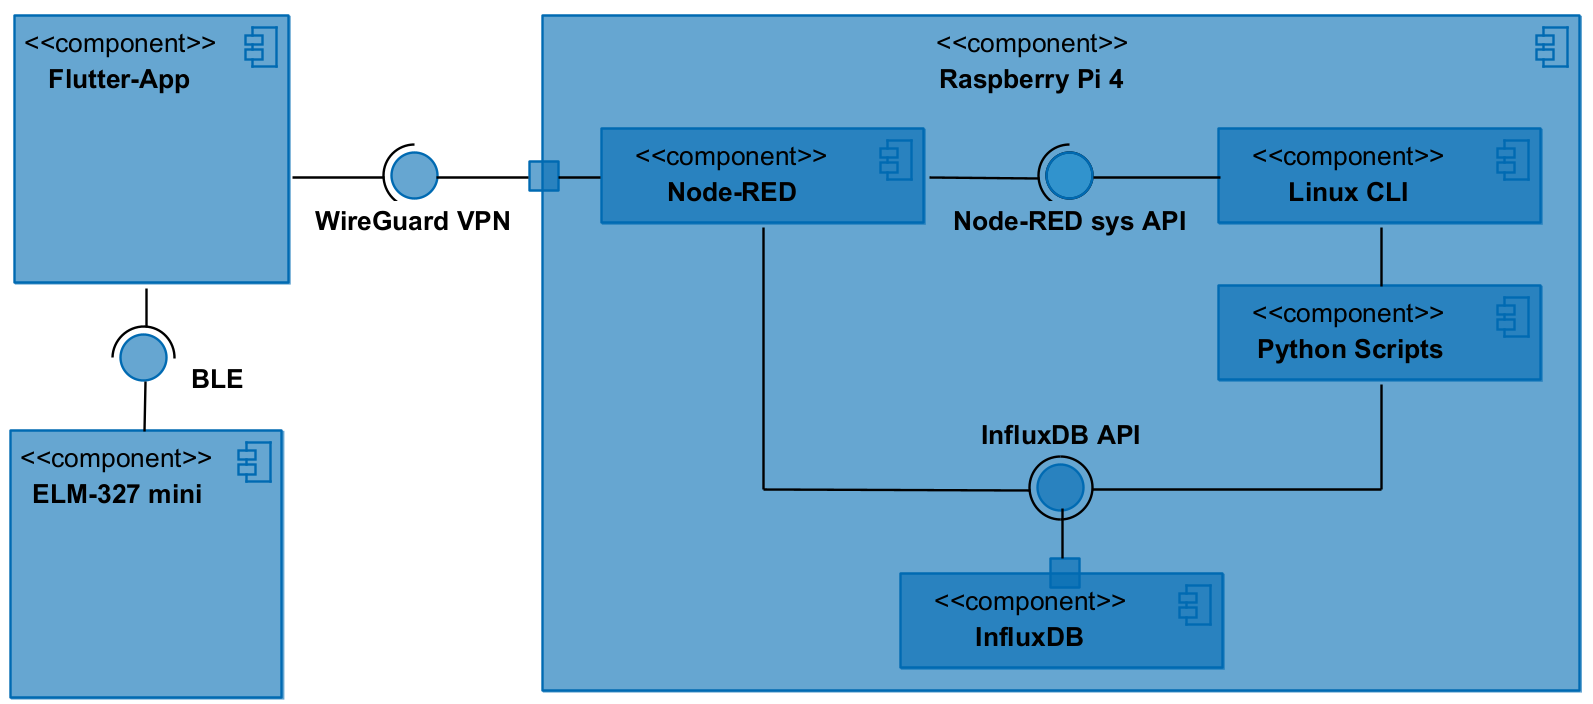
\includegraphics[width=0.95\textwidth]{images/component_diagramm_overview.png}
  \caption{Übersicht zur Architektur des Softwareprojekts}
  \label{fig:architecture}
\end{figure}

In der anderen Hälfte von Abbildung {\ref{fig:architecture}} ist ein weiteres Subsystem, in diesem Fall das auf einem Raspberry Pi 4 
umgesetzte Backend, abgebildet. Auf dem Raspberry Pi wurde der Container-Service Portainer installiert, welcher für die Verwaltung von 
Backend-Anwendungen wie beispielsweise dem Rapid-Prototyping-Framework Node-RED (Kapitel \ref{sec:foundations_nodered}) oder der 
Influx-Datenbank.
Wie in der Abbildung zu erkennen ist, nimmt Node-RED die leitende Rolle innerhalb des Backends ein, was bedeutet, dass die Mobile-App 
ausschließlich mit dieser Subkomponente über einen Port auf dem Raspberry Pi interagiert. Um eine zuverlässige Verbindung und einen 
sicheren Datenaustausch zwischen diesen beiden Ptoragonisten zu gewährleisten,
wird das WireGuard VPN (Virtual Private Network) verwendet. Dieser Prozess wird in Kapitel \ref{sec:implement_backend} noch genauer erläutert.
Aufgrund der verwaltenden Rolle, die das Framework übernimmt, verfügt Node-RED über Zugriff zu anderen Containern des Portainer-
Environments, um zum Beispiel über entsprechende APIs mit der Influx-Datenbank oder dem Command Line Input (CLI) des Raspberry Pi 
zu interagieren.

\section{Data Aquisition mit einer Smartphone-App}
\label{sec:implement_dataaquisition}

Um das Fahrverhalten eines Fahrers erfolgreich zu analysieren, müssen im Vorfeld Informationen zur Fahrt gesammelt werden. Um dies 
zu ermöglichen, wird festgelegt, welche Informations- oder Datentypen zu sammeln sind. Dabei muss nicht nur zwischen Datentypen, 
sondern auch zwischen dem Ursprung dieser Daten, also den Datenquellen, unterschieden werden. 
In diesem Projekt übernimmt die Applikation auf dem Smartphone die Aufgabe, OBD-II-Daten von dem entsprechenden Diagnose-Adapter 
abzurufen und diese um weitere essentielle Informationen zu ergänzen. Nach dem Sammeln eines vollständigen Fahrdatenbündels wird dieses 
in eine Datenstruktur sortiert, bevor es an das Backend vermittelt wird.
Im folgenden werden die im Rahmen dieses Projekts auftretenden Datenquellen aufgelistet und erläutert, welche Informationen auf welche
Weise erhoben werden.

\subsection*{ELM-327 OBD-II-Adapter}

Der OBD-II-Adapter ELM-327 (Kapitel \ref{subsec:foundations:elm327}) dient der Übermittling spezifischer Informationen während 
der Fahrt. Einzelne Datenpunkte können über den ELM-327 direkt bei dem Bordcomputer des Fahrzeugs abgefragt werden, indem an 
diesen eine aus zwei Hexadezimalzahlen bestehende Nachricht via Bluetooth Low Energy gesendet wird. Es gibt jedoch nicht nur die Möglichkeit,
Daten abzufragen, sondern auch direkt mit dem OBD-II-Adapter zu kommunizieren. Im unten aufgeführten Ausschnitt sind einige 
Beispielnachrichten zu sehen.

\begin{lstlisting}[language=Python, caption={Beispiel eines Requests für Echtzeit-Fahrdaten}]
  > atz
  < ELM327 v1.5

  > atsp6
  < OK

  > 01 0D
  < 41 0D 3A
\end{lstlisting}

Die beiden oberen Nachrichten werden verwendet, um den OBD-II-Adapter zu konfigurieren. Die Nachricht \textit{atz} wird verwendet,
um den Adapter zu kontaktieren und dessen Softwareversion abzufragen. Der Befehl \textit{atsp6} dient der Konfiguration des Nachrichtenprotokolls,
in diesem Fall ist das CAN-Bus Protokoll ausgewählt.
Die unten angeführte Nachricht zeigt die Abfrage von Echtzeitdaten des Fahrzeugs. Sie setzt sich zusammen aus dem Mode (in diesem Fall \textit{01}) der Nachricht und der 
eigentlichen Parameter-ID, auch PID genannt (hier \textit{0D}), des Datenpunktes, dessen Informationen abgefragt werden sollen.
\\
Im Folgenden werden die zu erhebenden OBD-II-Datenpunkte genauer erläutert:
\begin{itemize}
  \item \textbf{Umdrehungen pro Minute des Motors (PID: 0C)} \\ Der OBD-II-Parameter Engine RPM (Revolutions Per Minute) misst die Drehzahl 
  des Motors, also wie viele Umdrehungen die Kurbelwelle des Motors pro Minute macht. Dieser Wert gibt Auskunft über die aktuelle 
  Motorleistung und den Betriebszustand des Fahrzeugs. Eine höhere Drehzahl bedeutet in der Regel, dass der Motor härter arbeitet, 
  während eine niedrigere Drehzahl auf einen geringeren Arbeitsaufwand hinweist. Die Motor-Drehzahl ist ein wichtiger Indikator 
  für die Effizienz und die Belastung des Motors.
  \item \textbf{Motorlast (PID: 04)} \\ Die Motorauslast gibt an, wie stark der Motor im Verhältnis zu seiner maximalen 
  Leistungsfähigkeit bei der Kraftübertragung durch die Räder auf die Straße belastet wird. Dieser Wert wird als Prozentsatz
  dargestellt, wobei 0 Prozent bedeuten, dass der Motor gar nicht belastet ist, und 100 Prozent bedeuten, dass der Motor seine 
  maximale Leistung erbringt.
  Die Motorlastangabe berücksichtigt Faktoren wie die Drosselklappenstellung, die Motordrehzahl und den Luftmassenstrom
  um eine Einschätzung darüber zu geben, wie stark der Motor belastet wird. Ein hoher Wert weist auf eine starke 
  Beanspruchung hin, während ein niedriger Wert auf eine geringe Last hindeutet.
  \item \textbf{Fahrzeuggeschwindigkeit (PID: 13)} \\  Die Fahrzeuggeschwindigkeit wird vom Fahrzeugsteuergerät (ECU) erfasst und über 
  das OBD-II-System bereitgestellt. Die Geschwindigkeit wird in der Regel in Kilometern pro Stunde (km/h) oder Meilen pro 
  Stunde (mph) angezeigt, je nach Region und Fahrzeugkonfiguration. Dieser Parameter ist nützlich für Diagnosen und Überwachungen, 
  da er wichtige Informationen über das Fahrverhalten und die Bewegungsgeschwindigkeit des Fahrzeugs liefert.
  \item \textbf{Stellung des Gaspedals (PID: 11)} \\ Die Throttle Position oder Gaspedalstellung beschreibt die aktuelle Position
  des Drosselklappenpedals oder der Drosselklappe in einem Fahrzeug. Diese Position gibt an, wie weit das Gaspedal mit dem
  Fuß gedrückt ist, und wird von einem Sensor überwacht, der die Information an das Motorsteuergerät (ECU) weiterleitet.
  Der Parameter wird üblicherweise in Prozent angezeigt, wobei 0.0 ein unberührtes Gaspedal (keine Gasabgabe) bedeutet 
  und 1.0 auf ein voll belastetes Gaspedal hindeutet. Diese Information ist wichtig für die Motorsteuerung, um die Menge
  des eingespritzten Kraftstoffs und die Luftzufuhr entsprechend anzupassen und so die Leistung und Effizienz des Motors 
  zu optimieren.
\end{itemize}

\subsection*{Smartphone-App}
Neben der Kommunikation mit dem OBD-II-Adapter dient die Applikation auf dem Smartphone des Nutzers dem Zweck, die erhobenen
Fahrdaten um Mehrwert bringende Datenpunkte zu erweitern.
Hierbei ist stets zu beurteilen, welche erweiterten Erkenntnisse die Ergänzung bestimmter Informationen liefert 
und ob die Leistungsfähigkeit der Datenübertragung dadurch beeinflusst wird. Ein Beispiel hierfür wäre das Verwenden
einer API, die einen REST-Call (Abrufen von Daten eines Servers über eine HTTP-Anfrage) verwendet, was zu Verzögerungen
aufgrund von Verbindungs- und Übertragungszeiten führen kann.
\begin{itemize}
  \item \textbf{Universally Unique Identifier / UUID} \\ Eine UUID (Universally Unique Identifier) ist ein 
  standardisierter Identifikator, der innerhalb des Systems eindeutig ist. Sie wird verwendet, um den Ursprung 
  beziehungsweise den Erzeuger von Daten oder Objekten eindeutig zu kennzeichnen. UUIDs verhindern Kollisionen 
  durch ihre große Anzahl möglicher Kombinationen und sind daher ideal für die Identifikation von Datensätzen
  in verteilten Systemen. Die Einzigartigkeit von UUIDs garantiert, dass Daten über verschiedene Systeme oder Softwarekomponenten
  hinweg konsistent und zuverlässig identifiziert werden können.
  \item \textbf{Zeitstempel} \\ Der Mehrwert von Zeitstempeln liegt in der verbesserten Nachvollziehbarkeit und
  Analysefähigkeit der Fahrdaten. Sie ermöglichen es, zeitabhängige Muster zu erkennen und Korrelationen zwischen 
  verschiedenen Ereignissen zu identifizieren, wie beispielsweise Beschleinigungs-, Brems- oder Schaltvorgänge.
  \item \textbf{GPS-Koordinaten} \\ GPS-Koordinaten dienen der präzisen Geolokalisierung und Kontextualisierung 
  der geloggten Fahraktivitäten. Durch sie eröffnet sich die Möglichkeit, den exakten Standort eines Fahrzeugs zu
  jedem Zeitpunkt der Fahrt zu ermitteln, wodurch detaillierte Routeneigenschaften in die Analyse der Fahrdaten mit einbezogen
  werden können.
\end{itemize}

Die eigentliche Datenerhebung oder auch Data Aquisition von Fahrdaten übernimmt die Mobile-App, welche in Flutter
implementiert wurde. Um eine Datenerhebung durchzuführen, muss der Benutzer der Applikation zur Funktionalität 
\textit{Aufzeichnung starten} navigieren, welche direkt beim Start dieser zu sehen ist (Abbildung \ref{fig:app_home}).

\begin{figure}[h!]
  \begin{subfigure}{0.45\textwidth}
    \centering
    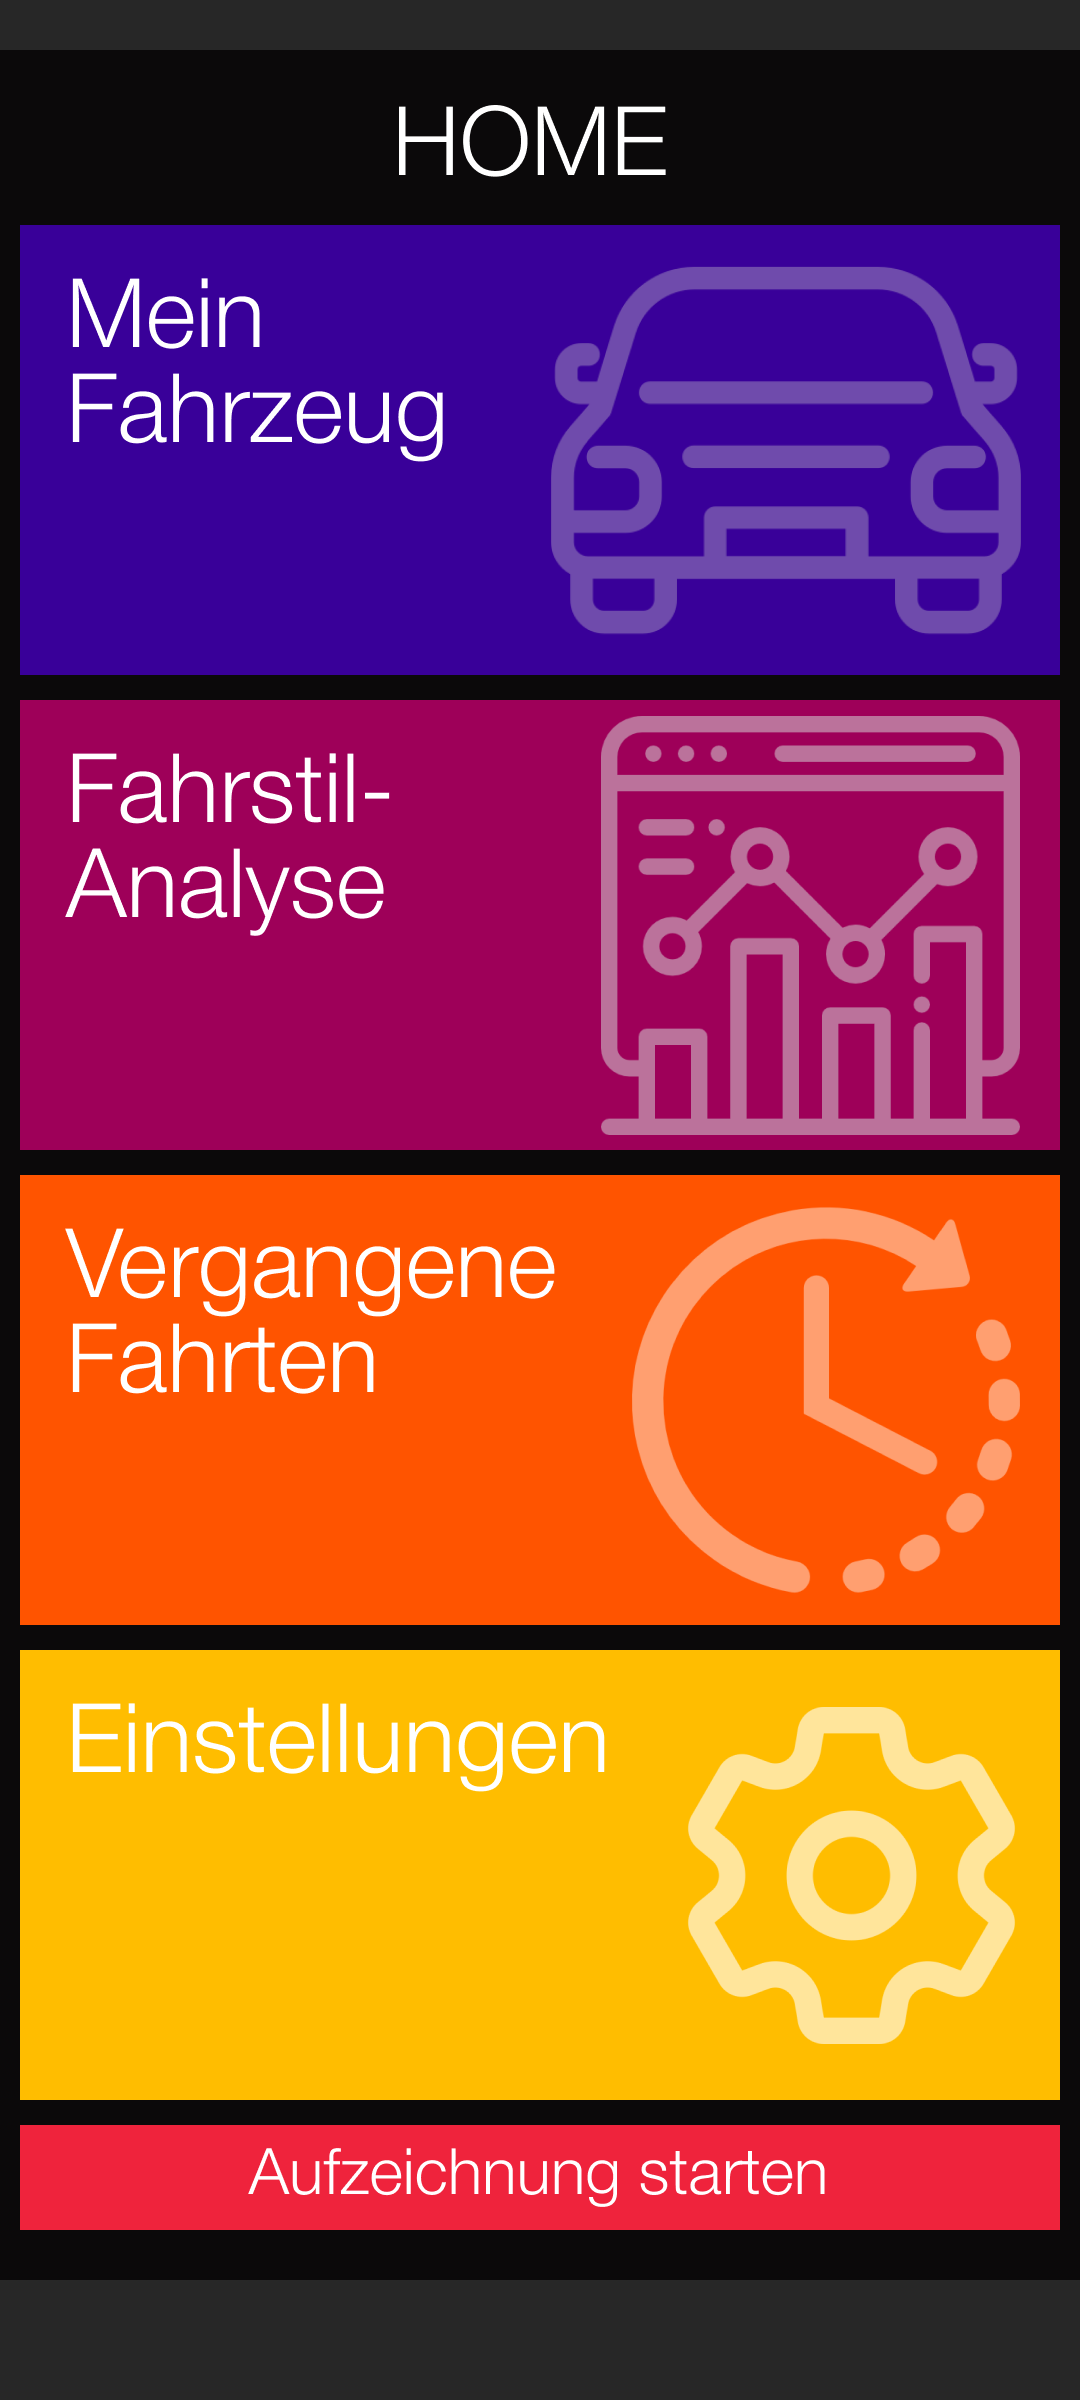
\includegraphics[width=0.45\linewidth]{images/app_conc_home.png}
    \caption{Startbildschirm der App CarSenseML}
    \label{fig:app_home}
  \end{subfigure}
  \begin{subfigure}{0.45\textwidth}
    \centering
    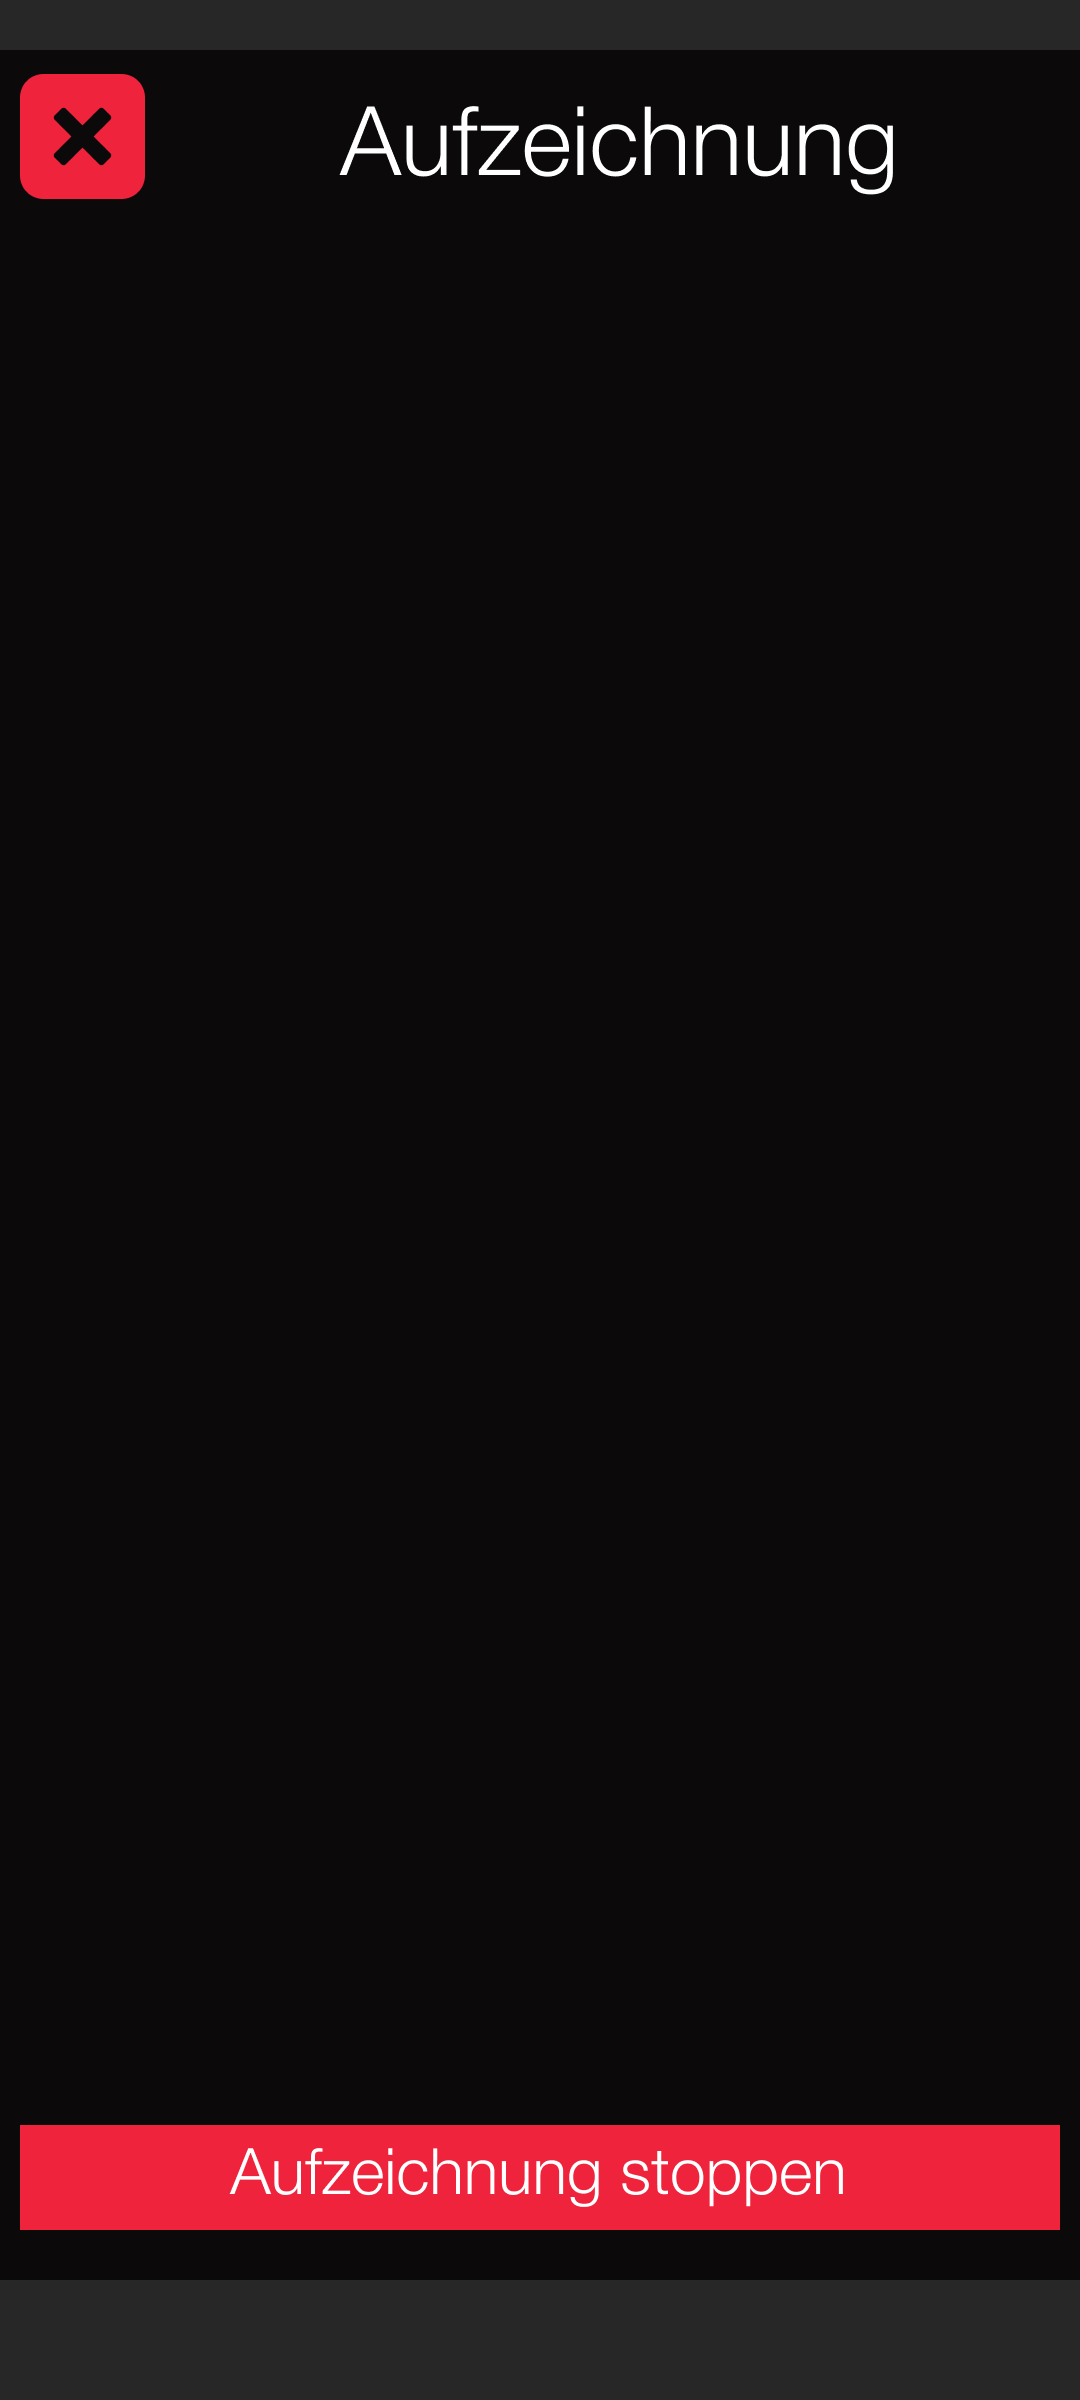
\includegraphics[width=0.45\linewidth]{images/app_conc_rec.png}
    \caption{Screen während der Datenerhebung}
    \label{fig:app_rec}
  \end{subfigure}
\end{figure}

Texttextblabla

\subsection*{Struktur der Fahrdatennutzlast}

\begin{verbatim}
  {
      "header": {
          "timestamp": "2024-06-18 13:46:22.853",
          "uudi": "f437137a-0d5b-46f7-b204-8ca4b94177aa",
          "type": 1
      },
      "payload": {
          "position": {
              "latitude": 48.840550,
              "longtitude": 10.068598
          },
          "travel_distance": 2.73,
          "vehicle_speed": 50,
          "engine": {
              "load": 0.46,
              "rpm": 3129,
              "coolant_temp": 78,
              "fuel_consumption_rt": 20.3
          },
          "driver": {
              "throttle_pos": 0.71
          }
      }
  }
  \end{verbatim}

\subsection*{Datenübertragung}

\section{Rapid-Prototyping-Backend auf einem Raspberry Pi}
\label{sec:implement_backend}

Für das Speichern der erhobenen Fahrdaten wurde ein Raspberry Pi 4 mit Linux-Betriebssystem aufgesetzt,
welcher die Rolle des Backends für das Projekt übernimmt. Um diese und weitere Funktionalitäten zu gewährleisten,
ist die Inbetriebnahme weiterer Services oder Docker-Container erforderlich. Ein Überblick zu dieser Architektur
ist in Abbildung \ref{fig:overview_backend} zu sehen.

\begin{figure}[h!]
  \centering
  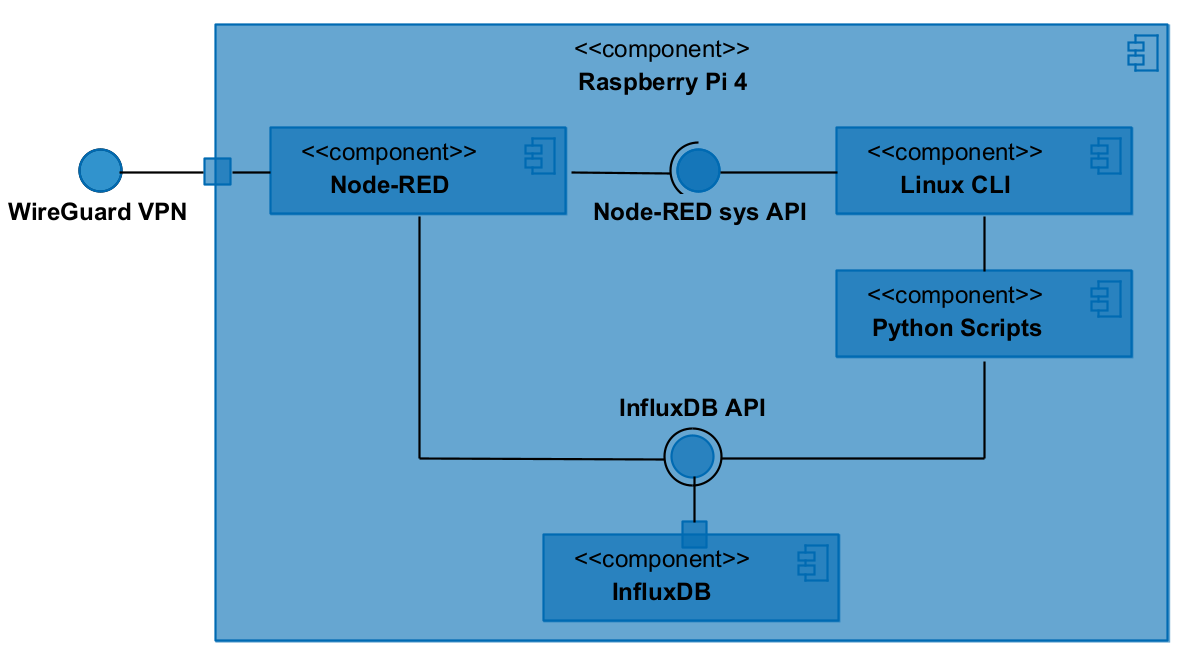
\includegraphics[width=0.95\textwidth]{images/comp_dia_raspi.PNG}
  \caption{Service- und Containerübersicht für den Raspberry Pi}
  \label{fig:overview_backend}
\end{figure}

\subsection*{WireGuard VPN}
Weil grundsätzlich davon auszugehen ist, dass Fahrdaten ausschließlich von außerhalb des Netzwerks, in dem sich 
das Backend befindet, an dieses gesendet werden, wurde ebenfalls ein WireGuard VPN in Betrieb genommen.
Die VPN-Software stellt eine abgesicherte Verbindung zu dem Netzwerk her, für das ein 
Verbindungszertifikat auf dem Smartphone angelegt wurde. Durch den sicheren VPN-Tunnel können das Backend und der Client 
- in diesem Fall die in Kapitel \ref{sec:implement_dataaquisition} beschriebene Smartphone-App - Nachrichten oder 
Nutzdaten austauschen.

\subsection*{Portainer als Container Management Software}
Weil grundsätzlich davon auszugehen ist, dass Fahrdaten ausschließlich von außerhalb des Netzwerks, in dem sich 
das Backend befindet, an dieses gesendet werden, wurde ebenfalls ein WireGuard VPN in Betrieb genommen.
Im Rahmen dieser Projektarbeit übernimmt Portainer die Aufgabe, die Services Node-RED und InfluxDB auszuführen
und zu verwalten.

\subsection*{Node-RED Framework}
Das Herzstück des Backends in dieser Projektarbeit ist ein mit dem Node-RED Framework implementierter Service,
über den sämtliche Funktionalitäten von diesem gesteuert werden.
Node-RED ist ideal für schnelles und unkompliziertes Prototyping, da es eine einfache und flexible Umgebung für
die Entwicklung von IoT- und Automatisierungslösungen bietet. WebSockets für die Echtzeitkommunikation,
HTTP-Requests für API-Aufrufe und Datenbank-APIs für die Anbindung und Abfrage von Datenbanken können mit Node-RED 
mühelos und mit geringem Zeitaufwand integriert und konfiguriert werden.


\section{Datengrundlage und Datenvorverarbeitung}
\label{sec:implement_dataprocessing}

\section{Fahrdatenanalyse mittels Machine Learning}
\label{sec:implement_Fahrverhaltensanalyse}

\subsection*{Data Labeling}

\subsection*{Machine Learning Model}

\subsection*{Hyperparameter Tuning}

\section{Smartphone-App - Subkomponente Ergebnisvisualisierung und E-Learning}
\label{sec:implement_elearning}

%---
\chapter{Evaluation}
\label{cha:evaluation}

%---
\chapter{Zusammenfassung und Ausblick}
\label{cha:zusammenfassung}

\section{Erreichte Ergebnisse}
\label{sec:ergebnisse}

\section{Fazit und Ausblick}
\label{sec:ausblick}

%-----------------------------------------------------------------------
\appendix

%---
\printbibliography[heading=bibintoc]

%---
\chapter{Anhang A}

\end{document}